\section{Einführung}\raggedbottom

\subsection{Motivation}
Im Rahmen der Projektarbeit soll ein verteilter \textit{in-memory storage} auf Basis von Apache Plasma entwickelt werden. Dieser verteilte Speicher soll in der Lage sein, große Datenmengen im Sinne von \textit{Big Data} zu speichern und zur Verfügung zu stellen.
 
Plasma ist Teil des Apache Arrow Projekts. Dieses Projekt beschreibt sein Einsatzgebiet wie folgt:
\begingroup
\addtolength\leftmargini{0.1in}
\begin{quote}
	``Apache Arrow defines a language-independent columnar memory format for flat and hierarchical data, organized for efficient analytic operations on modern hardware like CPUs and GPUs. The Arrow memory format also supports zero-copy reads for lightning-fast data access without serialization overhead.''\cite{Foundation}
\end{quote}
\endgroup
Der Zugriff erfolgt hierbei über Bibliotheken in diversen Programmiersprachen.
Hierbei sei zu beachten, dass Plasma selbst nicht als verteilte Anwendung konzipiert ist. Zwar können mehrere Instanzen auf einem Computer gestartet werden, jedoch verfügt Plasma über kein Protokoll, um mehrere Instanzen über ein Netzwerk zu verbinden. Somit ist auch der Speicher nicht verteilt und jeweils nur auf einem Computer verfügbar.

\subsection{Ziel}
Um die oben genannte Problematik zu lösen, soll ein Protokoll entwickelt werden, welches es ermöglicht mehrere Instanzen zu einem Netzwerk Cluster zu verbinden. Dieses Overlay-Netzwerk wird in Java entwickelt. Wie in Abbildung \ref{fig_Architektur} dargestellt, sind alle Komponenten miteinander verbunden. Wobei jeder Node und der Dispatcher jeweils eine direkte Verbindung zu allen anderen Komponenten des Netzwerks besitzt. Wenn Daten gespeichert werden sollen, entscheidet der Dispatcher, welcher Node für die Daten verantwortlich ist. Der Dispatcher nutzt Redis zur Datenhaltung.

\begin{figure}[htb]
	\begin{center}
		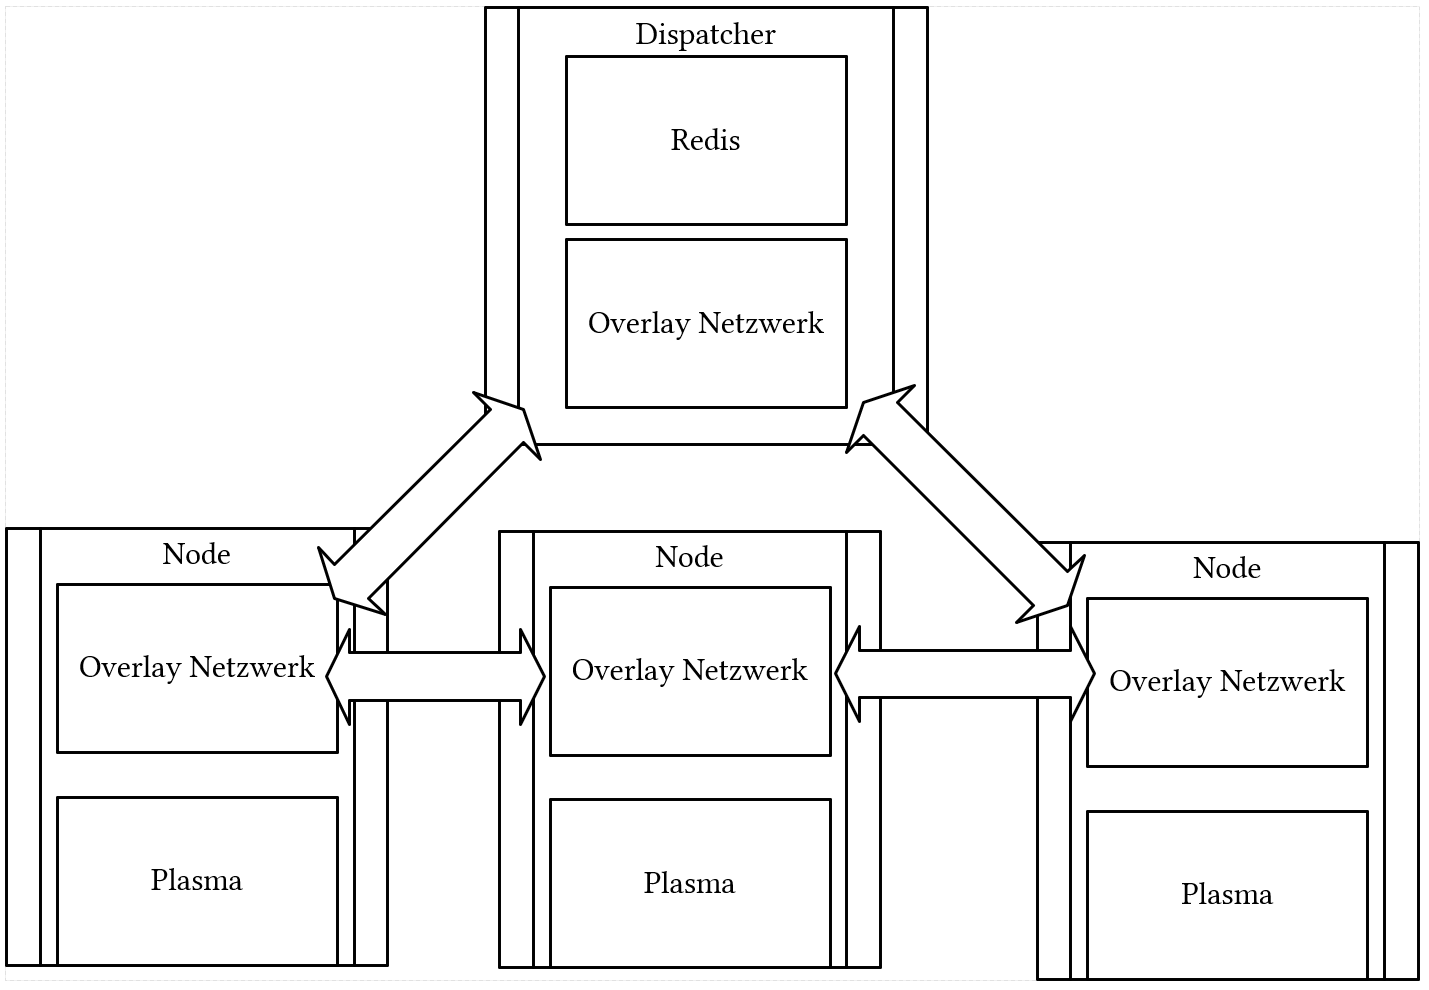
\includegraphics[width=0.8\textwidth]{bilder/Architektur.png}
		\caption{Skizze der angedachten Architektur.}\label{fig_Architektur}
	\end{center}
\end{figure}


\pagebreak
\section{Projektstufen}\raggedbottom
Die Projektarbeit gliedert sich in verschiedene, aufeinander folgende Phasen. Die Projektarbeit beginnt mit einem theoretischen Teil und endet mit einem praktischen Teil.
\subsection{Theoretischer Teil}
Dieser Teil beginnt mit der Anforderungsanalyse. Die hier beschriebene Software soll in ein bereits existierendes System integriert werden. Somit muss die Kompatibilität zu den bereits existierenden Komponenten in Form von Soft- und Hardware gewährleistet sein.
Darauf folgt der Entwurf der Anwendungsfälle. Hierbei gilt es Funktionalitäten zu beschreiben, die zwingend notwendig sind. Ergänzend dazu können noch weitere Funktionalitäten festgelegt werden, die zwar wünschenswert wären, aber nicht zwingend erforderlich sind. Danach muss die Architektur festgelegt und spezifiziert werden, um die Anwendungsfälle zu erfüllen. Verschiedene Lösungsansätze sollen beschrieben und verglichen werden.
\subsection{Praktischer Teil}
Basierend auf der Spezifikation werden die Komponenten implementiert. Zusätzlich sollen Tests und eine Dokumentation des Quellcodes erstellt werden. Die so erstellte Lösung soll in Hinblick auf wichtige Metriken wie IOPs, Bandbreite, Latenz etc. evaluiert werden.